\chapter{Flatland Environment}

Since we have solved the problem of railway scheduling on a railway line,
we want to use the knowledge developed
so far and work on \textbf{railway scheduling on a railway network}.
Recently, AICrowd developed a flatland environment[11] to foster progress in multi-
agent reinforcement learning for any re-scheduling problem (RSP). They have
defined the railway network in a complete new setting using grid instead of graph. Future
course of the project is to work on more general problem of flatland (which can be used for
solve railway scheduling, transport management problems) and develop algorithms that can
solve scheduling problem over grid world having multiple agents.

\vspace{\baselineskip}
This chapter contains flatland environment specifications and discusses about the problem statement in 
detail. Flatland is usually a two-dimensional environment intended for multi-agent problems, 
in particular it should serve as a benchmark for many multi-agent reinforcement learning approaches.
The environment can host a broad array of diverse problems reaching from disease spreading to train traffic management.
The flatland environment is a two-dimensional grid in which many agents can be placed,
and each agent must solve one or more navigational tasks in the grid world.

\section{Environment}
Flatland is grid-like n-dimensional space of any size. 
A cell is the elementary element of the grid. 
The cell is defined as a location where any objects can be located at. 
The term agent is defined as an entity that can move within the grid and must solve tasks.
 An agent can move in any arbitrary direction on well-defined transitions from cells to cell.
 The cell where the agent is located at must have enough capacity to hold the agent on. 
 Every agent reserves exact one capacity or resource. 
 The capacity of a cell is usually one. 
 Thus usually only one agent can be at same time located at a given cell. 
 The agent movement possibility can be restricted by limiting the allowed transitions.

 \vspace{\baselineskip}
 Flatland is a discrete time simulation. 
 A discrete time simulation performs all actions with constant time step. 
 In Flatland the simulation step moves the time forward in equal duration of time. 
 At each step the agents can choose an action. 
 For the chosen action the attached transition will be executed. 
 While executing a transition Flatland checks whether the requested transition is valid. 
 If the transition is valid the transition will update the agents position.
  In case the transition call is not allowed the agent will not move. 

\subsection{Tile types}
Each Cell within the simulation grid consists of a distinct tile type which in turn limit 
the movement possibilities of the agent through the cell. 
For railway specific problem 8 basic tile types can be defined which describe a rail network. 
As a general fact in railway network when on navigation choice must be taken at maximum two options 
are available.

\begin{figure}[h]
    \centering
    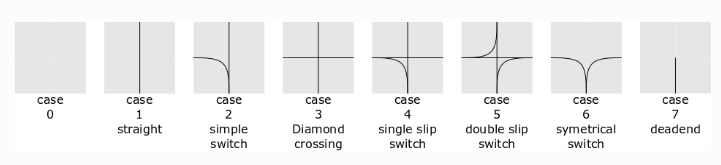
\includegraphics[width=1.0\textwidth]{flatland1}
    \caption{ Tile types in flatland grid \cite{WEBSITE:8} }
    \label{image-myimage2}
\end{figure}

\section {Observations}
In order to solve the flatland environment using RL, we need to decide the observation space and 
action space. Depending on the observation space, we can use different RL algorithms to solve.

\subsection{Global Observation}

Gives a global observation of the entire rail environment.
The observation is composed of the following elements:

\begin{itemize}
    \item Transition map array with dimensions (env.height, env.width, 16), assuming 16 bits encoding of transitions.
    \item Two 2D arrays (env.height, env.width, 2) containing respectively the position of the given agent target and the positions of the other agents targets.
    \item A 3D array (env.height, env.width, 8) with the first 4 channels containing the one hot encoding of the direction of the given agent and the second 4 channels containing the positions of the other agents at their position coordinates.
\end{itemize}

Global observations, specifically on a grid like environment, benefit from the vast research results 
on learning from pixels and the advancements in convolutional neural network algorithms. 
The observation can simply be generated from the environment state and not much additional 
computation is necessary to generate the state.
Also, in this case, when we consider global observation, it is like having a superagent (a 
central controler), which will take action for each of the trains after having the global 
observation.

\subsection{Tree Observations}
Tree observations are local observation that is made for each agent in the environment whenever agent
need to take the action. Also if we consider local observation of each agent then the environment becomes
multiagent, as opposed to the case of global observation.
The tree observation is built by exploiting the \textbf{graph structure of the railway network}. 
The observation is generated by spanning a 4 branched tree from the current position of the agent. 
Each branch follows the allowed transitions until a cell with multiple allowed transitions is reached. 
Here the information gathered along the branch is stored as a node in the tree. This is 
very similar to the observation we made in the previous chapters (in case of scheduling at railway line)
 where the observation is 
the resource information of the resource next to the train and at back to the train.
The figure below illustrates how the tree observation is built:

\begin{figure}[h]
    \centering
    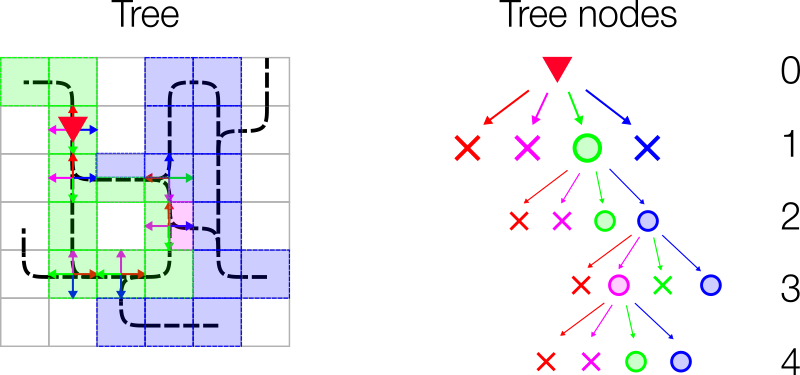
\includegraphics[width=1.0\textwidth]{flatland2}
    \caption{ Tree observation in flatland environment \cite{WEBSITE:8}}
    \label{image-myimage2}
\end{figure}

Each node is filled with information gathered along the path to the node. 
Each node contains 9 features:

\begin {enumerate}
\item If own target lies on the explored branch the current distance from the agent in number of cells is stored.
\item If another agent’s target is detected, the distance in number of cells from the current agent position is stored.
\item If another agent is detected, the distance in number of cells from the current agent position is stored.
\item Possible conflict detected.
\item If an unusable switch (for the agent) is detected we store the distance. An unusable switch is a switch where the agent does not 
have any choice of path, but other agents coming from different directions might.
\item This feature stores the distance (in number of cells) to the next node (e.g. switch or target or dead-end).
\item Minimum remaining travel distance from this node to the agent’s target given the direction of the agent if this path is chosen.
\item Agent in the same direction found on path to node.
\item Agent in the opposite direction on path to node.
\end{enumerate}

\section {Action space}
Thus the actions\cite{WEBSITE:8} of an agent are strongly limited to the railway network. 
This means that in many cases not all actions are valid. The possible actions of an agent are
\begin{enumerate}
    \item 0 \textbf{Do Nothing}: If the agent is moving it continues moving, if it is stopped it stays stopped
    \item 1 \textbf{Deviate Left}: If the agent is at a switch with a transition to its left, 
        the agent will chose th eleft path. Otherwise the action has no effect. 
        If the agent is stopped, this action will start agent movement again if allowed by the 
        transitions.
    \item 2 \textbf{Go Forward}: This action will start the agent when stopped. 
    This will move the agent forward and chose the go strai
    ght direction at switches.
    \item 3 \textbf{Deviate Right}: Exactly the same as deviate left but for right turns.
    \item 4 \textbf{Stop}: This action causes the agent to stop.
\end{enumerate}

\section{Problem Instances}
We can generate different problem instances in the flatland environment, with different railway network 
(sparse as well as dense), different schedules for the agent (trains).
We can also have different speed 
for each agent.
We can also mention the malfunction parameter for each train as this will control the 
rate at which a particular agent malfunctions. Also this will instroduce stochasticity in the environment.
For this work, we will be using three different problem instances as shown in the figure.


\begin{figure}[h]
    \centering
    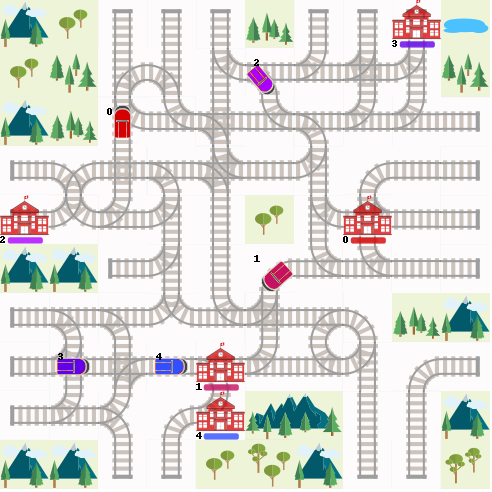
\includegraphics[width=0.5\textwidth]{flatland4}
    \caption{ A random environment. This is a toy example and minimum baseline for the algorithm\cite{WEBSITE:6} }
    \label{image-myimage2}
\end{figure}

\begin{figure}[h]
    \centering
    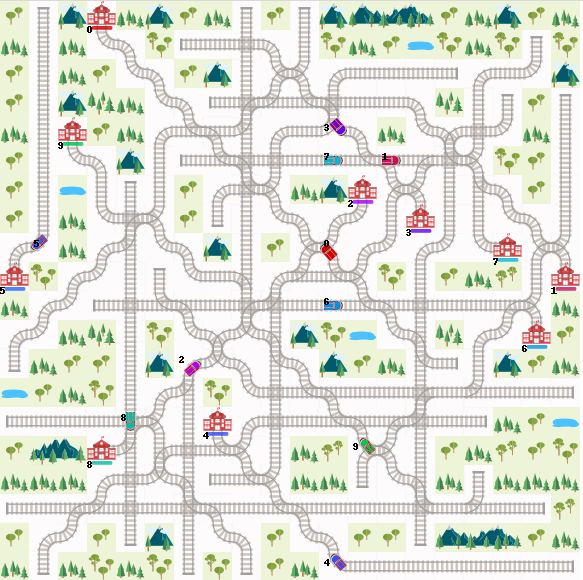
\includegraphics[width=0.5\textwidth]{flatland3}
    \caption{ A complex railway network. Due to the complexity of the network , there are 
    multiple paths from each agent position to their target. Even having multiple paths doen't make 
    this problem instance easy to solve\cite{WEBSITE:6}. }
    \label{image-myimage2}
\end{figure}


\begin{figure}[h]
    \centering
    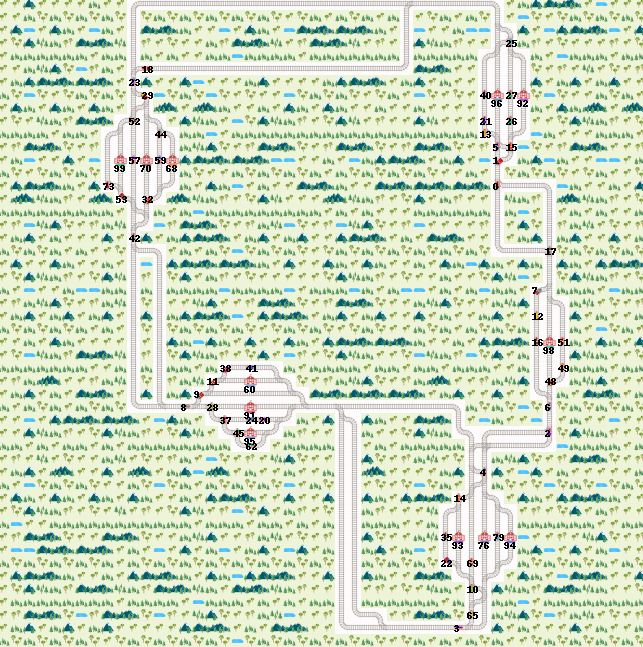
\includegraphics[width=0.8\textwidth]{flatland5}
    \caption{ Real life example.This example have 4 cities (where there are multiple parallel tracks and train targets 
    denoted by red house) each connected by two parallel railway lines. We can add to the complexity by increasing the
    number of cities, decreasing number of parallel track. Also the number of agents in this environment can be large 
    (like 100)\cite{WEBSITE:6} }
    \label{image-myimage2}
\end{figure}
